\documentclass[tikz]{standalone}
\usepackage{units}
\begin{document}

\tikzstyle{box} = [
  draw, minimum height = 1cm, minimum width = 1.5cm, fill=blue!20,
  rectangle, rounded corners, text centered]

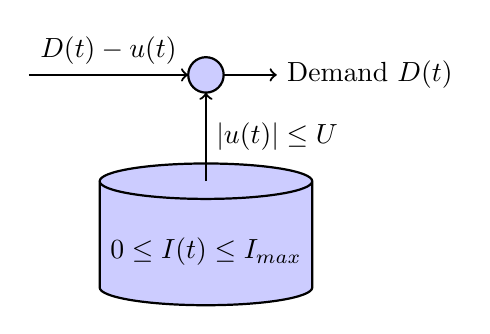
\begin{tikzpicture}[auto,thick,node distance = 1cm,scale = 0.9]
  %\draw [help lines] (-3,-1) grid (7,5);

  % Draw tank starting at upper left corner
  \draw [-,fill=blue!20] (1.5,1.5) 
    -- ++(0,-1.5) arc (-180:0:1.5 and 0.25) 
    -- ++(0,1.5) arc (0:360:1.5 and 0.25);
  \draw (3,0.5) node {$0 \leq I(t) \leq I_{max}$};

  % Draw flow junction
  \draw [-,thick,fill=blue!20] (3,3) circle (0.25);

  % Draw and label streams
  \draw [->,thick] (0.5,3) -- (2.75,3) 
    node [midway,above] {$D(t)-u(t)$};
  \draw [->,thick] (3,1.5) -- (3,2.75) 
    node [midway,right] {$|u(t)|\leq U$};
  \draw [->,thick] (3.25,3) -- (4,3) 
    node [right] {Demand $D(t)$};

\end{tikzpicture}

\end{document}